% !TEX encoding = UTF-8 Unicode
\documentclass[../天体物理基础.tex]{subfiles}
\begin{document}
\section{星系}
星系是由恒星、恒星残骸、星际气体与尘埃、暗物质等构成的引力束缚系统。

\subsection{银河系}
不识庐山真面目,只缘身在此山中。

1610 年,伽利略首先通过望远镜发现银河由无数恒星组成。1785 年,赫歇尔通过计量不同方向的恒星密度,得到第一幅银河系整体图像:银河系为扁盘状,太阳位于中心附近。1896\text{\textendash}1921 年,Kapteyn 利用照相底片测量不同天区的恒星密度,用统计视差求得恒星距离,首次估计银河系直径$\sim\qty{5e4}{ly}$,厚度$\sim\qty{1e4}{ly}$,他认为太阳位于银河系中心附近。

1920 年,Shapley 利用球状星团内的造父变星等测量星团距离,并给出球状星团的空间分布。Shapley 发现球状星团均匀地分布在银河的两侧,并且有向人马座聚集的倾向。

沙普利认为球状星团是银河系的子系统,并以银心为分布中心,由此估计太阳系到银心的距离为$\qty{5e4}{ly}$,在沙普利的模型中,银河系的结构是扁盘状的,直径$\qty{3e5}{ly}$.

早期对银河系的研究集中在可见光波段,由于天文学家并不了解星际介质的存在及其消光作用,因而得到关于银河系结构的错误的结论。

直到 20 世纪 30 年代人们才认识到星际介质的分布范围及其对观测的重要影响,并逐步发展了射电与红外的手段来研究银河系的结构。

\subsubsection{银河系的整体结构}
银河是天空中的一个环带,在人马座附近最亮、最宽,它的中心线近似为天球上的一个大圆。

银河系是一个直径约$20$万光年,包含约$1\text{\textendash}4\times10^{11}$课恒星,具有漩涡结构的盘状星系。

银河系可分为四个组成部分,分别是银盘 (disk),旋臂 (spiral arm), 核球 (bulge) 和银晕 (halo).

银盘呈扁盘状,包含年轻年老恒星、气体与尘埃,存在恒星形成,天体作圆轨道运动。核球呈花生状,位于银盘中心,包含年轻年老恒星、气体与尘埃,恒星整体无规则轨道运动,也有绕银心的轨道运动。银盘与核球存在恒星形成。银晕近似包裹住银盘的球形,只有年老恒星,无气体与尘埃,恒星形成已经停止了,恒星作无规则轨道运动。

银心定义为银河系的质心和动力学(转动)中心。由于射电源 Sgr A 的位置与旋转中性氢的动力学中心重合,1958 年 IAU 决定采用 Sgr A 的位置作为银河系中心。后来人们发现银河系中心有一超大质量黑洞,即射电源 Sgr A$^{*}$.

1944 年巴德 (Walter Baade) 发现星系晕与核球中的恒星明显比盘中的恒星颜色偏红,由此根据金属丰度的大小提出星族的概念。星族\uppercase\expandafter{\romannumeral1}是年轻的富金属恒星,主要位于银盘中,如疏散星团。星系盘中的星族\uppercase\expandafter{\romannumeral1}恒星绕银心作规则的圆轨道运动。星族\uppercase\expandafter{\romannumeral2}恒星是年老的贫金属恒星,主要位于银晕和核球中,如球状星团。恒星晕中星族\uppercase\expandafter{\romannumeral2}恒星的绕银心作高偏心率的椭圆轨道运动,且轨道取向是随机的。

金属丰度越低的恒星离银道面越远,这暗示了银河系的演化。

\subsubsection{银盘}
银河系的银盘分为薄盘加厚盘,恒星密度分布满足
\begin{equation}
n\left(R,z\right)\propto{}\left(\symup{e}^{-\left\vert{}z\right\vert{}/h_{\text{thin}}}+0.02\symup{e}^{-\left\vert{}z\right\vert{}/h_{\text{thick}}}\right)\symup{e}^{-R/h_{\text{R}}}.
\end{equation}

薄盘包含$\qty{6e10}{M_{\odot}}$的恒星和$\qty{0.5e10}{M_{\odot}}$的气体与尘埃,B 波段光度为$\qty{2e10}{L_{\odot}}$,质光比为 3.

厚盘恒星质量约$\qty{3e9}{M_{\odot}}$,B 波段光度$\qty{2e8}{L_{\odot}}$,质光比为 15.

通过测量太阳附近的恒星和气体云的视向速度和自行随银经的变化来判断恒星的轨道运动方式(如刚体转动还是较差转动)。在太阳周围$\ang{360;;}$的范围内,恒星的谱线位移表现出周期性的蓝移和红移。在太阳附近,距离银心越远,转动速度越小。

\begin{figure}[!htp]
\centering
\tikzset{every picture/.style={line width=0.75pt}}
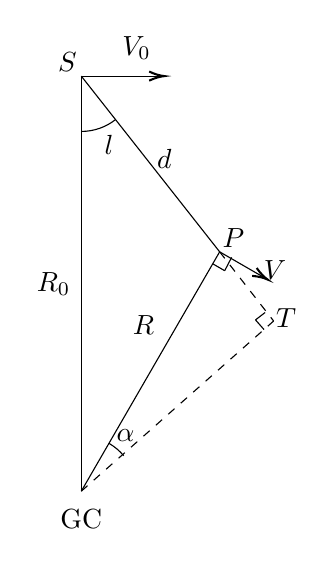
\begin{tikzpicture}[x = 0.5pt, y = 0.5pt, yscale = 1, xscale = 1]
\draw (0, 0) -- (0, 300);
\draw (0, -20) node {GC};
\draw (-10, 310) node {$S$};
\draw (-20, 150) node {$R_{0}$};

\draw (0, 300) -- (60, 300);
\draw [shift = {(60, 300)}, rotate = 180][line width = 0.75](10.93, -3.29) .. controls (6.95, -1.4) and (3.31, -0.3) .. (0, 0) .. controls (3.31, 0.3) and (6.95, 1.4) .. (10.93, 3.29);
\draw (40, 320) node {$V_{0}$};

\draw (0, 260) arc (-90:-52:40);
\draw (20, 250) node {$l$};

\draw (0, 0) -- (100, 173);
\draw (45, 120) node {$R$};

\draw (100, 173) -- (134.6, 153);
\draw [shift = {(134.6, 153)}, rotate = 150][line width = 0.75](10.93, -3.29) .. controls (6.95, -1.4) and (3.31, -0.3) .. (0, 0) .. controls (3.31, 0.3) and (6.95, 1.4) .. (10.93, 3.29);
\draw (110, 183) node {$P$};
\draw (140, 160) node {$V$};
\draw (95, 164.35) -- (103.65, 159.35);
\draw (108.65, 169) -- (103.65, 159.35);

\draw [dashed](0, 0) -- (139, 123);
\draw (148, 125) node {$T$};
\draw [dashed](100, 173) -- (139, 123);
\draw (132.05, 116.85) -- (125.9, 123.8);
\draw (132.85, 129.15) -- (125.9, 123.8);

\draw (0, 300) -- (100, 173);
\draw (60, 240) node {$d$};

\draw (20, 34.6) arc (60:40:40);
\draw (32, 40) node {$\alpha$};
\end{tikzpicture}
\captionsetup{justification=raggedright, singlelinecheck=false}
\caption{Oort 公式图示。}
\label{Oort 公式图示。}
\end{figure}

设银经为$l$的恒星和太阳的转动角速度分别为$\omega=\dfrac{V}{R}$和$\omega_{0}=\dfrac{V_{0}}{R_{0}}$,恒星相对于太阳的视向速度为$V_{\text{r}}=V\cos\alpha-V_{0}\sin l$.几何关系$\cos\alpha=\dfrac{R_{0}\sin l}{R}$.

那么视向速度为$V_{\text{r}}=R_{0}\left(\omega-\omega_{0}\right)\sin l$,切向速度为$V_{\text{t}}=R\omega\sin\alpha-R_{0}\omega_{0}\cos l$,几何关系$R\sin\alpha=R_{0}\cos l-d,d$为恒星到太阳的距离,那么切向速度为$V_{\text{t}}=R_{0}\left(\omega-\omega_{0}\right)\cos l-\omega d$

在$R=R_{0}$附近将$\omega-\omega_{0}$泰勒级数展开,
\begin{equation}
\omega-\omega_{0}=\left(\frac{\symup{d}W}{\symup{d}R}\right)_{R_{0}}\left(R-R_{0}\right)+\cdots\approx\frac{1}{R_{0}^{2}}\left[R_{0}\left(\frac{\symup{d}V}{\symup{d}R}\right)_{R_{0}}-V_{0}0\right]\left(R-R_{0}\right),
\end{equation}
对$R\approx R_{0}\gg d,R-R_{0}\approx-d\cos l$有
\begin{equation}
V_{\text{r}}=Ad\sin2l,V_{\text{t}}=Ad\cos2l+Bd,
\end{equation}
根据太阳附近恒星的视向和切向速度,可以求出奥尔特常数:
\begin{align}
A&=\frac{1}{2}\left[\frac{V_{0}}{R_{0}}-\left(\frac{\symup{d}V}{\symup{d}R}\right)_{R_{0}}\right]\approx\qty{15}{km\cdot{}s^{-1}\cdot kpc^{-1}}.\notag\\
B&=-\frac{1}{2}\left[\frac{V_{0}}{R_{0}}+\left(\frac{\symup{d}V}{\symup{d}R}\right)_{R_{0}}\right]\approx\qty{-14}{km\cdot{}s^{-1}\cdot{kpc^{-1}}}.
\end{align}
从而求出太阳绕银心转动角速度$\omega_{0}=A-B=29\pm\qty{1.8}{km\cdot{}s^{-1}\cdot kpc^{-1}}$,转动周期约$\qty{2.2e8}{yr}$,转动速度约$238\pm\qty{15}{km\cdot{}s^{-1}}$.上述数据是本地静止标准速度,太阳相对于该速度还有约$\qty{10}{km\cdot{}s^{-1}}$的本动速度。

银河系自转曲线和质量分布

测量方法:

$R<R_{0}$时测量视线方向上$\ce{H}\,\symup{\uppercase\expandafter{\romannumeral1}}$谱线和$\ce{CO}$谱线的最大位移,从而测得最大视向速度,而速度满足$V_{\text{r}}=R\left(\omega-\omega_{0}\right),R=R_{0}\sin l$,进而得到$\omega\left(R\right)$和$V\left(R\right)$.

$R>R_{0}$时观察$\ce{H}\,\symup{\uppercase\expandafter{\romannumeral2}}$区的发射线、分子云的$\ce{CO}$分子毫米波谱线和 Maser 谱线测定视向速度,利用$V_{\text{r}}=R_{0}\left(\omega-\omega_{0}\right)\sin l$确定$\omega$,利用$\ce{H}\,\symup{\uppercase\expandafter{\romannumeral2}}$区内的高温恒星确定距离,进而确定$\omega\left(R\right)$.或者或者利用甚长基线干涉技术测量 Maser 的自行,如果还能确定距离,就能计算$V_{\text{t}}$和$\omega\left(R\right)$.

最后发现自转曲线内区刚体转动,外区较为平坦。太阳轨道内包含的质量为
\begin{equation}
M=\frac{R_{0}V_{0}^{2}}{\symup{G}}\sim\qty{e11}{M_{\odot}},
\end{equation}
银河系可见质量约$\qty{6e10}{M_{\odot}}$.约$\qty{e12}{M_{\odot}}$,最可能的解释是银晕中存在大量的暗物质。

银河系旋臂的证认

光学观测:

示踪天体:OB 型星,年轻的疏散星团、发射星云和$\ce{H}\,\symup{\uppercase\expandafter{\romannumeral2}}$区、经典造父变星

限制:星际尘埃消光

射电观测:

示踪天体:$\ce{H}\,\symup{\uppercase\expandafter{\romannumeral1}}$区、分子云

方法:测量$\qty{21}{cm}$谱线和分子云毫米波谱线的多普勒位移,与银河系自转曲线比较,从而得到距离、甚长基线三角视差法

限制:气体云的转动是非圆的,在圆运动的同时还有无规则运动

观测结果

天鹅臂、英仙臂、猎户臂、人马臂、盾牌{}-{}南十字臂、矩尺臂

旋臂理论解释

首先旋臂不是物质臂。一方面旋臂存在时间较长,如果旋臂由同样的物质构成,较差自转会使旋臂缠绕或消失。另一方面表征旋臂的主要是年轻天体,恒星寿命有限,也会导致旋臂消失。

1963 年林家翘和徐瑕生提出密度波理论,认为旋臂实际上是密度波的表现。星系引力势的扰动使天体运动速度发生变化,天体轨道取向相互耦合使物质密度规则变化,从而使密度波在银盘内传播,产生对称的整体旋臂。

旋臂密度波漩涡图样绕银心刚体转动,$\omega=\qty{13.5}{km\cdot{}s^{-1}\cdot{}kpc^{-1}}$.在银河系内区天体的运动速度超过旋涡图样速度,在外区天体比旋涡图样运动得更慢。气体云接近旋臂后碰撞坍缩,形成恒星。

此外还有一种自传播恒星形成理论:气体云坍缩引发的热星辐射和超新星爆发产生激波,压缩周围气体,引发下一代恒星诞生,天体绕银心较差转动形成旋臂。这种方式形成的旋臂维持时间较短,形状也较粗糙。

\subsubsection{核球和银晕}
银河系中心区域是大小约$6\times\qty{4}{kpc}$的棒状结构,核心是盒形/花生形的核球,恒星分布十分密集,密度比太阳附近高$10^{5}$倍,质量约$\qty{e10}{M_{\odot}}$.

光学波段,核球附近区域受到星际气体和尘埃的强烈消光,因此红外和射电波段是研究银心的主要途径。

银心区域充满相对论电子和磁场,具有强烈的射电辐射。银心周围$\qty{10}{pc}$区域,电离气体与尘埃组成微型漩涡结构。银心周围$\qty{100}{pc}$区域,延展的纤维状气体与银道面垂直,反映了银心区域的磁力线。

费米泡?

恒星晕:包含球状星团与晕星。星族\uppercase\expandafter{\romannumeral2}恒星以银心为中心球状分布,在椭圆轨道上绕银心旋转,质量约占星系恒星总质量的$1\%$.

气体晕:弥漫的 X 射线辐射表明在银晕中存在大量的热气体 ($T\sim\qty{e6}{K}$),质量约$\left(2.5\pm1\right)\times\qty{e10}{M_{\odot}}$

暗物质晕:由银河系的自转曲线得知,银晕中的不可见物质质量远超过银河系可见物质质量。暗物质在所有波段都不产生辐射、仅有引力与弱相互作用。

暗物质可能的成分:

1. MACHOs (Massive Compact Halo Objects), 包括褐矮星、行星、中子星、黑洞等。

2. WIMPs (Weakly Interacting Massive Particles), 亚原子非重子物质。

可以利用微引力透镜研究暗物质含量。可以研究 WIMPs 与原子核碰撞产生的热辐射,两个 WIMPs 湮灭产生的次级粒子(伽马射线,正电子,中微子等)。

\subsubsection{银河系的起源}

pdf84 ©C. Chiappini 有两幅图描绘星系图景,可以抄一下。

Conroy et al. arViv:2204.02989 有一副晕、厚盘、薄盘元素丰度的图

中小质量恒星演化产生$\ce{C,N}$, 产生行星状星云。大质量恒星演化产生\uppercase\expandafter{\romannumeral1}b, \uppercase\expandafter{\romannumeral1}c, \uppercase\expandafter{\romannumeral2}型超新星,产生$\ce{O}$,白矮星双星演化产生\uppercase\expandafter{\romannumeral1}a 型超新星,产生$\ce{Fe}$.

记得把这段移到恒星中 pass

整体坍缩模型:银河系起源于一个几百万光年大小的原初气体云。气体云沿转动轴方向坍缩,通过耗散过程形成扁平盘,在大约 2 亿年内形成致密核球和转动的气体薄盘。与此同时,气体在坍缩过程中形成球状星团和第一代恒星。这些天体继承了坍缩云块的运动特征,表现为晕星的无规则运动。大质量恒星发生超新星爆发,气体中重元素增丰。第二代恒星开始在盘上形成,具有规则的圆轨道特征。后面形成的恒星有越来越高的金属丰度。

问题:

该模型预言自外向内恒星年龄和金属丰度的连续变化,但是银河高纬度地区有金属丰度反常的恒星

晕中的恒星有净的反向转动速度

球状星团的年龄比该模型预言的要高一个量级。

并合和吸积模型:银河系由许多小星系并合而成。原初的小团块已经经历了不同程度的恒星形成和演化过程,因此具有不同的金属丰度。星系盘是通过持续的并合和吸积过程形成的——当吸积气体向内运动时,径向运动的耗散和环向运动的加速导致气体盘的形成。

近年来巡天观测发现,银河系厚盘形成于 130 亿年前。110 亿年前,银河系与一矮星系并合,形成了内晕。接下来的五六十亿年中,银河系经历持续的金属元素富集。形成厚盘的气体在 80 亿年前耗尽,新的气体开始从银河系周围聚集,银河系薄盘恒星开始形成并持续至今。

\subsection{星系概述}
可观测宇宙中大约有$10^{11}\text{\textendash}10^{12}$个星系,亮度限制的样本中,椭圆星系、漩涡星系、不规则星系的比例分别为$20\%,77\%,3\%$.体积限制的样本中三者比例分别为$12\%,34\%,54\%$.

\paragraph{椭圆星系}~{}

除中心核区外无其他结构,没有星系盘,主要由星族\uppercase\expandafter{\romannumeral2}恒星构成,没有或仅有少量星际气体和尘埃,颜色偏红。恒星作无规则的椭圆轨道运动。近 10 亿年没有明显的恒星形成。

星系中心最亮,亮度向边缘递减。我们可以用面亮度(单位平方角秒的星等)描述亮度,多数椭圆星系满足
\begin{equation}
I\left(R\right)=I_{0}\exp\left[-7.67\left(\frac{R}{R_{\text{e}}}\right)^{\frac14}\right],
\end{equation}

\paragraph{漩涡星系}~{}

中心是球状或椭球状的核球。外面是扁平的星系盘,从核球两端延伸出两条或以上的螺旋状旋臂。盘外面是球状的星系晕。星系盘,特别是旋臂上主要是星族\uppercase\expandafter{\romannumeral1}恒星及气体和尘埃。核球和星系晕主要由星族\uppercase\expandafter{\romannumeral2}恒星构成,气体和尘埃很少。星系盘颜色偏蓝,星系晕和核偏红。盘中恒星和气体作圆轨道运动,晕中恒星作无规则轨道运动。旋臂中有恒星形成。

同样有面亮度分布,不过椭圆星系是$\exp\left(-\left(\dfrac{R}{R_{\text{e}}}\right)^{\frac14}\right)$,盘星系是$\exp\left(-\left(\dfrac{R}{R_{\text{e}}}\right)\right)$.

Faber-Jackson 关系

\paragraph{棒漩星系}~{}

旋臂起源于棒的两端。

\subsubsection{测量星系}
我们关心星系的距离、大小、质量、形态、光度、颜色、金属丰度、恒星形成历史。

光度函数:星系在绝对光度间隔范围内的数目。假设球状星团的光度函数是普适的,通过比较遥远星系中球状星团的流量分布和定标星系中球状星团的光度分布确定距离。

漩涡星系谱线位移转化为自转速度转化为质量

椭圆星系速度弥散转化为质量

\subsection{星系集团}

\subsubsection{本星系群}

大小约$\qty{3}{Mpc}$,包含至少 54 个成员星系,其中 3 个是漩涡星系,其他是不规则星系和矮椭圆星系。银河系和仙女座星系 M31 是最大的两个星系,大部分小星系被引力束缚在它们周围。

大麦哲伦云$D=\qty{50}{kpc},M=\qty{2e10}{M_{\odot}},d=\qty{10}{kpc}$. SMC: $D=\qty{60}{kpc},M=\qty{4e9}{M_{\odot}},d=\qty{6}{kpc}$.均为不规则星系,绕银河系转动,富含年轻恒星和中性气体。

麦哲伦流:跨越天空$\ang{180;;}$,连接银河系和麦哲伦云的高速 ($\qty{400}{km\cdot{}s^{-1}}$) 气体流,产生于银河系与麦哲伦云之间的潮汐作用。

M31 是本星系群中最大的星系,$M\sim\qty{1.5e12}{M_{\odot}}$,距离$\sim\qty{770}{kpc}$,直径$\sim\qty{60}{kpc}$, Sb 型漩涡星系,正在接近银河系。

M33 是本星系群中第三大星系,$M\sim\qty{5e10}{M_{\odot}}$,距离$\sim\qty{720}{kpc}$,直径$\sim\qty{18}{kpc}$, Sc 型漩涡星系,拥有大量星族\uppercase\expandafter{\romannumeral1}天体和恒星形成区。

星系团

包含至少$50$个明亮星系的集团。富星系团至少上千。

室女星系团是距离最近的星系团,$D\sim\qty{16.5}{Mpc}$,直径$\sim\qty{4}{Mpc}$,包含至少 2500 个星系。致密核区由早型星系主导,周围是延展分布的旋涡星系。

后发星系团距离$\sim\qty{100}{Mpc}$,直径$\sim\qty{3}{Mpc}$,包含约 6700 个成员星系,其中绝大部分是漩涡星系,其他为椭圆星系。

可以在位力平衡下根据星系团的大小和成员星系的运动速度可以得到星系团的引力质量:
\begin{equation}
M\sim\frac{RV^{2}}{\symup{G}}.
\end{equation}

X 射线观测发现星系团中温度达到$\qty{e7}{K}$的热气体,星系团的可见质量不足以束缚这些气体。根据引力透镜现象可以估计星系团的引力质量,发现同样远远超过星系团中所有可见物质质量。

星系之间的相互作用是十分普遍的。哈勃空间望远镜的深场观测在$\qty{e3}{Mpc}$处发现大量年轻的不规则小星系,表面 100 亿年前星系间相互作用是十分普遍的。

星系之间的相互作用为扰动和并合,会影响漩涡结构、尘埃带和恒星的形成。影响相互作用强度的因素包括:星系的质量比、星系的相对运动速度、星系间的距离。根据星系大小,并合可分为主并合和次并合。根据气体含量,并合可分为干并合和湿并合。

观测证据?

超星系团

由几十到几百个星系团组成,典型尺度为$\qty{100}{Mpc}$,质量$\qty{e16}{M_{\odot}}$.

由于宇宙膨胀和星系团相互间较弱的引力,处于膨胀或松散束缚状态,在宇宙空间呈网状相互连接。

宇宙大尺度结构

在$>\qty{100}{Mpc}$的尺度上进行星系红移巡天,同时观测上千个星系的光谱以测量它们的距离,发现宇宙中的物质分布呈现一种泡沫网状结构:几乎所有的星系都分布在狭窄的纤维带上,只占据$1\text{\textendash}2\%$的空间,在它们之间是巨大的空洞,典型尺度为$50\text{\textendash}100$万光年,其中的星系极少。

星系起源于宇宙大爆炸后的初始密度扰动

引力不稳定性导致暗物质晕生成

重子物质成团和坍缩

形成第一代恒星和星系

恒星形成和演化的 feedback, 星系间的相互作用,中心大质量黑洞的形成及其反馈会改变星系形态

时间越早,星系的形态越不规则,盘星系和椭圆星系在更低的红移处开始主导。

星系的并合比例随红移的增加而增大。

自上而下:热暗物质主导的宇宙中,热暗物质的动能可以在小尺度上抵抗引力的压迫。原始气体坍缩首先产生巨大的薄饼状结构,然后薄饼沿一个方向坍缩,变成巨大的丝状结构。这些结构由于引力不稳定性再次碎裂成更小尺度的结构。

自下而上:冷暗物质主导的宇宙中,先形成较小的星系,再慢慢并合。

大质量星系的形成早于小质量星系。

大质量星系中的恒星形成更早、持续时间更短。


%\printbibliography

\end{document}